% Stationary battery CDF, lambda=3 (theta=0)
% Requires: \usepackage{pgfplots}, \pgfplotsset{compat=1.18}
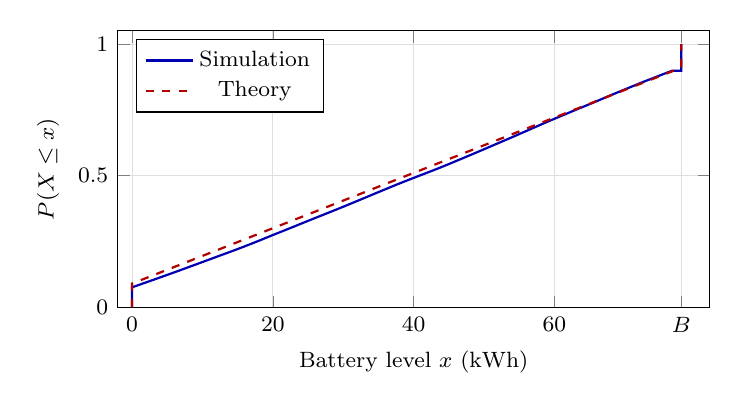
\begin{tikzpicture}
  \begin{axis}[
    width=0.75\textwidth, height=0.42\textwidth,
    xmin=-2, xmax=82, ymin=0, ymax=1.05,
    xlabel={Battery level $x$ (kWh)},
    ylabel={$P(X \leq x)$},
    legend pos=north west,
    legend style={font=\footnotesize},
    grid=major, grid style={gray!25, line width=0.3pt},
    tick label style={font=\footnotesize},
    label style={font=\footnotesize},
    xtick={0,20,40,60,78},
    xticklabels={0,20,40,60,$B$},
  ]
  \addplot[blue!70!black, thick] coordinates {
    (0.0000,0.0)  
    (0.0000,0.07579)
    (1.3220,0.08825)
    (2.6441,0.10071)
    (3.9661,0.11319)
    (5.2881,0.12587)
    (6.6102,0.13853)
    (7.9322,0.15162)
    (9.2542,0.16451)
    (10.5763,0.17752)
    (11.8983,0.19063)
    (13.2203,0.20362)
    (14.5424,0.21660)
    (15.8644,0.23007)
    (17.1864,0.24402)
    (18.5085,0.25818)
    (19.8305,0.27266)
    (21.1525,0.28671)
    (22.4746,0.30092)
    (23.7966,0.31522)
    (25.1186,0.32964)
    (26.4407,0.34383)
    (27.7627,0.35786)
    (29.0847,0.37207)
    (30.4068,0.38643)
    (31.7288,0.40099)
    (33.0508,0.41575)
    (34.3729,0.43061)
    (35.6949,0.44524)
    (37.0169,0.45984)
    (38.3390,0.47408)
    (39.6610,0.48800)
    (40.9831,0.50169)
    (42.3051,0.51534)
    (43.6271,0.52912)
    (44.9492,0.54355)
    (46.2712,0.55831)
    (47.5932,0.57314)
    (48.9153,0.58802)
    (50.2373,0.60312)
    (51.5593,0.61834)
    (52.8814,0.63349)
    (54.2034,0.64861)
    (55.5254,0.66416)
    (56.8475,0.67962)
    (58.1695,0.69516)
    (59.4915,0.71039)
    (60.8136,0.72525)
    (62.1356,0.74009)
    (63.4576,0.75485)
    (64.7797,0.76931)
    (66.1017,0.78409)
    (67.4237,0.79909)
    (68.7458,0.81384)
    (70.0678,0.82844)
    (71.3898,0.84295)
    (72.7119,0.85724)
    (74.0339,0.87097)
    (75.3559,0.88471)
    (76.6780,0.89839)
    (78, 0.89839)
    (78.0000,1.00000)
  };
  \addlegendentry{Simulation};
  \addplot[red!70!black, dashed, thick] coordinates {
    (0.0000,0.0)
    (0.0000,0.09009)
    (1.3220,0.10399)
    (2.6441,0.11788)
    (3.9661,0.13178)
    (5.2881,0.14567)
    (6.6102,0.15957)
    (7.9322,0.17346)
    (9.2542,0.18736)
    (10.5763,0.20125)
    (11.8983,0.21515)
    (13.2203,0.22904)
    (14.5424,0.24294)
    (15.8644,0.25683)
    (17.1864,0.27073)
    (18.5085,0.28462)
    (19.8305,0.29852)
    (21.1525,0.31241)
    (22.4746,0.32631)
    (23.7966,0.34020)
    (25.1186,0.35410)
    (26.4407,0.36800)
    (27.7627,0.38189)
    (29.0847,0.39579)
    (30.4068,0.40968)
    (31.7288,0.42358)
    (33.0508,0.43747)
    (34.3729,0.45137)
    (35.6949,0.46526)
    (37.0169,0.47916)
    (38.3390,0.49305)
    (39.6610,0.50695)
    (40.9831,0.52084)
    (42.3051,0.53474)
    (43.6271,0.54863)
    (44.9492,0.56253)
    (46.2712,0.57642)
    (47.5932,0.59032)
    (48.9153,0.60421)
    (50.2373,0.61811)
    (51.5593,0.63200)
    (52.8814,0.64590)
    (54.2034,0.65980)
    (55.5254,0.67369)
    (56.8475,0.68759)
    (58.1695,0.70148)
    (59.4915,0.71538)
    (60.8136,0.72927)
    (62.1356,0.74317)
    (63.4576,0.75706)
    (64.7797,0.77096)
    (66.1017,0.78485)
    (67.4237,0.79875)
    (68.7458,0.81264)
    (70.0678,0.82654)
    (71.3898,0.84043)
    (72.7119,0.85433)
    (74.0339,0.86822)
    (75.3559,0.88212)
    (76.6780,0.89601)
    (78.0000,0.90991)
    (78.0000,1.0)
  };
  \addlegendentry{Theory};
  \end{axis}
\end{tikzpicture}